% =====================================================================
%  V2V-Project -- Study Pack
%  Section S4 : The 4-Step Authentication Handshake
%  Source file studied: protocol/auth_protocol.py
%  Standalone document -- compile with:  pdflatex 04-authentication-handshake.tex
% =====================================================================
\documentclass[11pt,a4paper]{article}

\usepackage[utf8]{inputenc}
\usepackage[T1]{fontenc}
\usepackage{lmodern}

\usepackage[a4paper,margin=2.4cm]{geometry}
\usepackage{enumitem}
\setlist{topsep=2pt,itemsep=2pt}

\usepackage{amsmath}
\usepackage{amssymb}
\usepackage{booktabs}
\usepackage{graphicx}
\usepackage{xcolor}
\usepackage{listings}
\usepackage{tikz}
\usetikzlibrary{arrows.meta,positioning,shapes.geometric,calc,fit,backgrounds}
\usepackage[colorlinks=true,linkcolor=blue,urlcolor=blue,citecolor=blue]{hyperref}

\definecolor{codebg}{rgb}{0.97,0.97,0.94}
\definecolor{codegreen}{rgb}{0.00,0.50,0.00}
\definecolor{codegray}{rgb}{0.50,0.50,0.50}
\definecolor{keyblue}{rgb}{0.00,0.20,0.70}
\definecolor{boxblue}{rgb}{0.88,0.93,1.00}
\definecolor{boxyellow}{rgb}{1.00,0.97,0.85}

\lstdefinestyle{py}{
  language=Python,
  backgroundcolor=\color{codebg},
  basicstyle=\ttfamily\footnotesize,
  keywordstyle=\color{keyblue}\bfseries,
  stringstyle=\color{codegreen},
  commentstyle=\color{codegray}\itshape,
  numberstyle=\tiny\color{codegray},
  numbers=left,
  numbersep=8pt,
  showstringspaces=false,
  breaklines=true,
  breakatwhitespace=false,
  frame=single,
  rulecolor=\color{codegray},
  tabsize=4,
  captionpos=b,
}
\lstdefinestyle{term}{
  backgroundcolor=\color{codebg},
  basicstyle=\ttfamily\footnotesize,
  breaklines=true,
  frame=single,
  rulecolor=\color{codegray},
  numbers=none,
  captionpos=b,
}

\title{\textbf{V2V-Project Study Pack}\\[4pt]
       \large Section S4 --- The 4-Step Authentication Handshake}
\author{Information Security Project --- Beginner Study Notes}
\date{Source file: \texttt{protocol/auth\_protocol.py}}

\begin{document}
\maketitle
\tableofcontents
\newpage

% =====================================================================
\section{Title and ``What You'll Learn''}
% =====================================================================

\subsection*{Section Title}
\textbf{S4 --- The 4-Step Mutual Authentication Handshake: how two vehicles
prove who they are to \emph{each other} and secretly agree on a session key.}

\subsection*{Plain-English Summary (read this first)}
Before two cars exchange a single safety message, they perform a
\emph{handshake} --- a short, fixed conversation in four steps. By the end of it
each car is sure of two things: (1) the other car is genuine (its certificate is
real \emph{and} it actually owns the matching private key), and (2) both cars now
hold an identical secret key that was \emph{never sent over the network}. The
handshake is built from a \textbf{HELLO}, a \textbf{CHALLENGE}, a
\textbf{RESPONSE} and an \textbf{ACK}. It is implemented by one file,
\texttt{protocol/auth\_protocol.py}, which stitches together the certificates of
Section~S2 and the cryptographic tools of Section~S3.

\subsection*{Learning Outcomes}
After studying this section you will be able to:
\begin{itemize}
  \item Explain \textbf{mutual authentication} and why one-sided authentication
        is not enough.
  \item Explain \textbf{challenge--response} and the role of the 32-byte
        handshake \textbf{nonce}.
  \item Explain how the \textbf{ReplayCache} and \textbf{TimestampValidator}
        block replayed handshake messages.
  \item Describe the four messages --- HELLO, CHALLENGE, RESPONSE, ACK --- and
        the data each carries.
  \item Walk through every method of the \texttt{AuthProtocol} class step by step.
  \item Explain how the same session key is derived on both sides via ECDH+HKDF.
  \item Run the handshake demo, read its log, and force it to fail in three
        different ways (stale message, replayed nonce, bad signature).
\end{itemize}

% =====================================================================
\section{Where This Fits}
% =====================================================================

S4 \emph{is} Stage~2 (Authentication) of the pipeline. It is the bridge: it
consumes the certificates created in Stage~1 (S2) and the cryptographic toolbox
of S3, and it produces the \textbf{session key} that Stage~3 (S5, secure
messaging) needs. Without a completed handshake there is no key, and without a
key no BSM can be encrypted.

\begin{center}
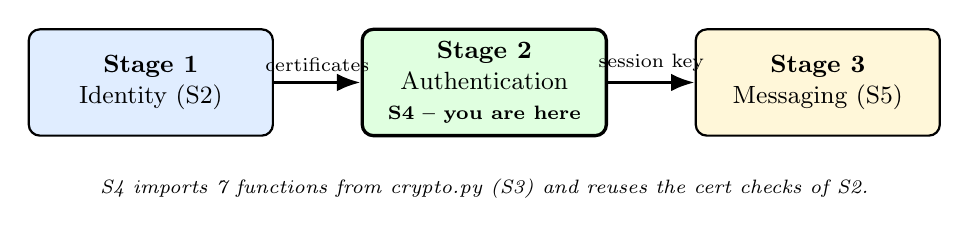
\begin{tikzpicture}[node distance=9mm and 11mm,every node/.style={font=\small},
    stage/.style={draw,rounded corners,minimum width=3.1cm,minimum height=1.35cm,
                  align=center,thick}]
  \node[stage,fill=boxblue]   (id)   {\textbf{Stage 1}\\Identity (S2)};
  \node[stage,fill=green!12,very thick,right=of id]   (auth)
       {\textbf{Stage 2}\\Authentication\\\scriptsize \textbf{S4 -- you are here}};
  \node[stage,fill=boxyellow,right=of auth] (msg) {\textbf{Stage 3}\\Messaging (S5)};
  \draw[-{Latex[length=3mm]},very thick] (id)   -- (auth)
       node[midway,above,font=\scriptsize]{certificates};
  \draw[-{Latex[length=3mm]},very thick] (auth) -- (msg)
       node[midway,above,font=\scriptsize]{session key};
  \node[below=4mm of auth,font=\scriptsize\itshape,align=center]
       {S4 imports 7 functions from crypto.py (S3) and reuses the cert checks of S2.};
\end{tikzpicture}
\end{center}

% =====================================================================
\section{The Theory You Must Study}
% =====================================================================

\subsection{Mutual Authentication}
\textbf{Plain definition.} \emph{Authentication} is proving who you are.
\emph{Mutual} authentication means \emph{both} parties prove their identity to
each other --- not just one side.

\textbf{Real-life analogy.} When you log in to a bank website, normally only
\emph{you} prove who you are (your password). Mutual authentication is stronger:
it is like meeting a courier where the courier shows you ID \emph{and} you show
the courier ID --- neither hands anything over until both are satisfied.

\textbf{Why it exists.} If only Vehicle~B checked Vehicle~A, an attacker could
impersonate B. If only A checked B, an attacker could impersonate A. A
man-in-the-middle relies on each side failing to check the other. Mutual
authentication closes both doors at once.

\textbf{How it works here.} In the handshake, B verifies A's certificate
\emph{and} A's signature, and A verifies B's certificate \emph{and} B's
signature. Both directions are checked before any safety message flows.

\textbf{Security property it provides.} \textbf{Authentication} (and, by
defeating MITM, it protects \textbf{confidentiality} and \textbf{integrity} too).

\subsection{Challenge--Response and the Handshake Nonce}
\textbf{Plain definition.} A \emph{challenge--response} is a test: one party
sends a fresh random value (the \emph{challenge}); the other must perform an
operation on it that only the genuine party could perform (the \emph{response}).
The fresh random value is a \textbf{nonce}.

\textbf{Real-life analogy.} A bouncer says ``say today's password backwards''.
Only someone who truly knows the password can do it, and because the request is
new each time, an eavesdropper who recorded yesterday's answer cannot reuse it.

\textbf{Why it exists.} Showing a certificate only proves the certificate is
real --- it does \emph{not} prove the sender \emph{owns} the matching private
key. A certificate is public; an attacker could copy it. The challenge--response
forces the sender to \emph{use} its private key on a value it could not have
predicted, proving live possession of the key.

\textbf{How it works here.} Each vehicle generates a 32-byte random nonce
(\texttt{os.urandom(32).hex()}). Each then \emph{signs} the pair of nonces with
its certificate private key (\texttt{ecdsa\_sign}). The other side verifies that
signature with the public key from the certificate (\texttt{ecdsa\_verify}). A
valid signature over a \emph{freshly chosen} nonce proves: ``you are online now
and you hold the private key''.

\textbf{Note on two kinds of nonce.} This 32-byte handshake nonce is \emph{not}
the same as the 12-byte AES-GCM nonce of S3. The handshake nonce is a freshness
challenge; the AES-GCM nonce makes each encryption unique. Same word, two jobs.

\textbf{Security property it provides.} \textbf{Authentication} and
\textbf{replay prevention}.

\subsection{Replay Attacks and the Replay Cache}
\textbf{Plain definition.} A \emph{replay attack} re-sends a previously captured,
genuine message. The \texttt{ReplayCache} is an in-memory list of nonces already
seen; a repeat is rejected.

\textbf{Real-life analogy.} A nightclub that ink-stamps each ticket as it is
used. A photocopied ticket carries a stamp number the door already recorded ---
entry refused.

\textbf{Why it exists.} Even a perfectly genuine, correctly signed HELLO becomes
dangerous if an attacker can record it and replay it later to start a bogus
session. The cache guarantees each nonce is accepted \emph{at most once}.

\textbf{How it works here.} \texttt{ReplayCache.check\_and\_add(nonce)} raises
\texttt{ReplayError} if the nonce is already stored, otherwise stores it with an
expiry of \texttt{now + 300\,s}. Old entries are cleaned out automatically. 300
seconds (5 minutes) is the constant \texttt{REPLAY\_WINDOW\_SECONDS}.

\textbf{Security property it provides.} \textbf{Replay prevention}.

\subsection{Timestamp / Freshness Validation}
\textbf{Plain definition.} Every handshake message carries the time it was
created. The \texttt{TimestampValidator} rejects any message whose time is too
far from ``now''.

\textbf{Real-life analogy.} A concert ticket printed with a date. The usher
glances at it: yesterday's ticket is refused on sight, without even checking the
seat number.

\textbf{Why it exists.} The replay cache only remembers nonces for 5 minutes and
costs memory. The timestamp check is a cheap first filter: a message hours old is
thrown out instantly. The two together are belt-and-braces.

\textbf{How it works here.} \texttt{TimestampValidator.validate(timestamp)}
computes \texttt{age = abs(now - timestamp)} and raises \texttt{StaleMessageError}
if \texttt{age > 5.0} seconds. Note the \texttt{abs}: a timestamp from the
\emph{future} is rejected too, which guards against clock-skew tricks.

\textbf{Security property it provides.} \textbf{Replay prevention}.

\subsection{Certificate Verification (recap from S2)}
The handshake must check that the certificate a peer presents was really signed
by the trusted CA. S4 does this with the helper
\texttt{verify\_certificate\_against\_ca}, which (1) parses the peer and CA
certificates, (2) verifies the CA's ECDSA-SHA256 signature on the peer
certificate, (3) checks the validity dates, and (4) returns the peer's public
key. This is the same logic explained fully in Section~S2 ---
S4 simply \emph{calls} it at the right moment. \emph{Security property:}
\textbf{authentication}.

\subsection{ECDH Ephemeral Key Exchange (recap from S3)}
During the handshake each vehicle generates a \emph{fresh} ECDH key pair
(\texttt{generate\_ecdh\_keypair}), sends the public half inside RESPONSE or ACK,
and combines its private half with the peer's public half
(\texttt{ecdh\_shared\_secret}) to get a shared secret. Both sides then run
\texttt{derive\_session\_key} (HKDF) to turn that secret plus the two nonces into
the \emph{same} 32-byte AES key. Because the ECDH keys are ephemeral, the session
has \textbf{forward secrecy}. The maths is covered in Section~S3.

\subsection{Dataclasses and the JSON Wire Format}
\textbf{Plain definition.} A Python \texttt{@dataclass} is a small class that
just holds named fields. \emph{JSON} (JavaScript Object Notation) is a simple
text format for structured data --- the form the messages take while crossing
the network.

\textbf{Real-life analogy.} A dataclass is a labelled paper form with named
boxes; \texttt{to\_json} folds the form into an envelope of text; \texttt{from\_json}
opens the envelope and reads the boxes back.

\textbf{Why it exists.} A network carries bytes, not Python objects. Each message
class has \texttt{to\_json()} (object $\to$ text) and \texttt{from\_json()} (text
$\to$ object), so a message can be sent and faithfully rebuilt on the far side.

\textbf{How it works here.} \texttt{HelloMessage}, \texttt{ChallengeMessage},
\texttt{ResponseMessage} and \texttt{AckMessage} are dataclasses. Each carries a
\texttt{msg\_type} tag (\texttt{"HELLO"}, \texttt{"CHALLENGE"}, ...) so the
receiver knows which form it has been handed. Binary values (nonces, signatures)
are carried as \emph{hex strings} because raw bytes cannot live inside JSON text.

\textbf{Security property it provides.} None directly --- it is the
\emph{format}, not a defence.

\subsection{Why Exactly Four Steps?}
Each step has a job, and you cannot remove one:
\begin{enumerate}
  \item \textbf{HELLO} --- A introduces itself and sends its certificate + nonce.
        (B can now check A's identity.)
  \item \textbf{CHALLENGE} --- B sends its certificate + nonce \emph{and} a
        signature over both nonces. (A can now check B's identity \emph{and}
        that B holds its private key.)
  \item \textbf{RESPONSE} --- A signs both nonces too, and sends its ephemeral
        ECDH public key. (B can now check A holds its key, and start the key
        exchange.)
  \item \textbf{ACK} --- B sends its ephemeral ECDH public key. (A can now finish
        the key exchange.)
\end{enumerate}
Steps 1--2 exchange certificates; steps 2--3 are the two-way challenge--response;
steps 3--4 exchange the ECDH public keys. Four messages is the minimum for
\emph{mutual} authentication plus a key agreement.

% =====================================================================
\section{Code Walkthrough}
% =====================================================================

\texttt{auth\_protocol.py} has four parts: custom exceptions, four message
dataclasses, two small protection classes (\texttt{ReplayCache},
\texttt{TimestampValidator}), the certificate helper, and the main
\texttt{AuthProtocol} class.

\subsection{The custom exceptions}
\begin{lstlisting}[style=py,caption={auth\_protocol.py --- the exception hierarchy.}]
class AuthError(Exception):
    """Base exception for authentication errors."""

class ReplayError(AuthError):
    """Raised when a replayed nonce is detected."""

class StaleMessageError(AuthError):
    """Raised when a message timestamp is too old."""

class CertificateError(AuthError):
    """Raised when certificate verification fails."""
\end{lstlisting}
\textbf{Explanation:} \texttt{AuthError} is the parent; the three children name
the three specific ways a handshake can be rejected --- a replayed nonce, a stale
message, a bad certificate. Naming each one separately makes the failure reason
obvious in logs and in the attack demos.

\subsection{The four message dataclasses}
\begin{lstlisting}[style=py,caption={auth\_protocol.py --- the HELLO message (the
other three messages follow the same pattern).}]
@dataclass
class HelloMessage:
    vehicle_id: str
    certificate_pem: str
    nonce: str
    timestamp: float
    msg_type: str = "HELLO"

    def to_json(self) -> str:
        return json.dumps(asdict(self))

    @classmethod
    def from_json(cls, data: str) -> HelloMessage:
        return cls(**json.loads(data))
\end{lstlisting}
\textbf{Step by step:}
\begin{enumerate}
  \item The \texttt{@dataclass} decorator auto-generates the boring boilerplate
        (constructor, etc.) so the class is just a list of named fields.
  \item \texttt{HelloMessage} fields: the sender's \texttt{vehicle\_id}, its
        \texttt{certificate\_pem} (its passport as text), its \texttt{nonce}
        (32 random bytes as a 64-character hex string), the \texttt{timestamp},
        and a fixed \texttt{msg\_type} tag.
  \item \texttt{to\_json} turns the object into a JSON text string ready to send.
  \item \texttt{from\_json} is a \emph{classmethod} that rebuilds the object from
        a received JSON string.
\end{enumerate}
The other three dataclasses differ only in their fields:
\begin{itemize}
  \item \texttt{ChallengeMessage} adds \texttt{signed\_nonces} (an ECDSA
        signature over both nonces, as hex).
  \item \texttt{ResponseMessage} carries \texttt{signed\_nonces} and
        \texttt{ecdh\_public\_key\_pem} (the ephemeral ECDH public key) ---
        note it has \emph{no} certificate field, because A already sent its
        certificate in HELLO.
  \item \texttt{AckMessage} carries only \texttt{ecdh\_public\_key\_pem} and a
        \texttt{session\_established} flag --- and, unlike the others, it has
        \emph{no timestamp field}.
\end{itemize}

\subsection{ReplayCache --- catching repeated nonces}
\begin{lstlisting}[style=py,caption={auth\_protocol.py --- the replay cache.}]
class ReplayCache:
    def __init__(self, window_seconds: int = 300) -> None:
        self._window = window_seconds
        self._seen: dict[str, float] = {}   # {nonce_hex: expiry_timestamp}

    def check_and_add(self, nonce: str) -> None:
        self._cleanup()
        if nonce in self._seen:
            raise ReplayError(f"Nonce already seen: {nonce[:16]}...")
        self._seen[nonce] = time.time() + self._window

    def _cleanup(self) -> None:
        now = time.time()
        expired = [n for n, exp in self._seen.items() if exp < now]
        for n in expired:
            del self._seen[n]
\end{lstlisting}
\textbf{Step by step:}
\begin{enumerate}
  \item \texttt{\_\_init\_\_} sets the remembering window (default 300\,s) and an
        empty dictionary \texttt{\_seen} mapping each nonce to the time it should
        be forgotten.
  \item \texttt{check\_and\_add} first calls \texttt{\_cleanup}.
  \item If the nonce is already in \texttt{\_seen}, it raises \texttt{ReplayError}
        --- this is a replay attack being caught.
  \item Otherwise it records the nonce with expiry \texttt{now + 300\,s}.
  \item \texttt{\_cleanup} deletes nonces whose expiry has passed, so the cache
        does not grow forever.
\end{enumerate}
\textbf{Arguments:} \texttt{nonce} (hex string). \textbf{Returns:} nothing.
\textbf{Exceptions:} \texttt{ReplayError}. \emph{Analogy:} the ink-stamp register
at the nightclub door.

\subsection{TimestampValidator --- catching stale messages}
\begin{lstlisting}[style=py,caption={auth\_protocol.py --- the timestamp validator.}]
class TimestampValidator:
    def __init__(self, max_age_seconds: float = 5.0) -> None:
        self._max_age = max_age_seconds

    def validate(self, timestamp: float) -> None:
        age = abs(time.time() - timestamp)
        if age > self._max_age:
            raise StaleMessageError(
                f"Message is {age:.1f}s old (max {self._max_age}s)"
            )
\end{lstlisting}
\textbf{Step by step:}
\begin{enumerate}
  \item \texttt{\_\_init\_\_} stores the maximum allowed age (default 5.0\,s).
  \item \texttt{validate} computes the \emph{absolute} difference between now and
        the message's timestamp.
  \item If that age exceeds 5 seconds, it raises \texttt{StaleMessageError}.
\end{enumerate}
\textbf{Why \texttt{abs}?} It rejects both \emph{too-old} messages (a real replay)
and \emph{too-future} messages (a forged or clock-skewed timestamp).
\emph{Analogy:} the usher refusing a ticket whose date is not today.

\subsection{verify\_certificate\_against\_ca --- the certificate gate}
\begin{lstlisting}[style=py,caption={auth\_protocol.py --- verify a peer certificate against the trusted CA.}]
def verify_certificate_against_ca(cert_pem, ca_cert_pem):
    try:
        cert_bytes = cert_pem.encode("utf-8") if isinstance(cert_pem, str) else cert_pem
        cert = x509.load_pem_x509_certificate(cert_bytes)
        ca_cert = x509.load_pem_x509_certificate(ca_cert_pem)

        # Verify the CA's signature on the vehicle certificate.
        ca_public_key = ca_cert.public_key()
        ca_public_key.verify(
            cert.signature,
            cert.tbs_certificate_bytes,
            ec.ECDSA(hashes.SHA256()),
        )

        # Check validity dates (now must be inside the window).
        now = datetime.now(timezone.utc)
        nb = getattr(cert, "not_valid_before_utc", None) or \
             cert.not_valid_before.replace(tzinfo=timezone.utc)
        na = getattr(cert, "not_valid_after_utc", None) or \
             cert.not_valid_after.replace(tzinfo=timezone.utc)
        if now < nb: raise CertificateError("Certificate is not yet valid")
        if now > na: raise CertificateError("Certificate has expired")

        pub_key = cert.public_key()
        if not isinstance(pub_key, ec.EllipticCurvePublicKey):
            raise CertificateError("Certificate does not contain an EC public key")
        return pub_key
    except CertificateError:
        raise
    except Exception as exc:
        raise CertificateError(f"Certificate verification failed: {exc}") from exc
\end{lstlisting}
\textbf{Step by step:}
\begin{enumerate}
  \item Parse the peer's certificate and the CA's certificate from PEM text.
  \item \texttt{ca\_public\_key.verify(...)} checks the CA's ECDSA-SHA256
        signature on the peer certificate's \texttt{tbs\_certificate\_bytes}
        (the ``to-be-signed'' body). A forged certificate fails here.
  \item Check that ``now'' is inside the certificate's validity window;
        otherwise raise \texttt{CertificateError}.
  \item Confirm the embedded public key is an elliptic-curve key, then
        \textbf{return} it --- the caller needs it to verify signatures.
  \item Any failure becomes a \texttt{CertificateError}.
\end{enumerate}
\textbf{Theory link:} certificate verification / chain of trust (S2). This is the
first of the two identity checks; the second is the signature challenge.

\subsection{The AuthProtocol class}

\subsubsection*{\_\_init\_\_ --- set up one vehicle's handshake state}
The constructor stores the vehicle's id, its private key, its certificate (PEM
bytes), and the CA certificate. It creates one \texttt{ReplayCache} and one
\texttt{TimestampValidator}, and prepares empty ``slots'' for the handshake
state: \texttt{my\_nonce}, \texttt{peer\_nonce}, \texttt{peer\_public\_key},
\texttt{session\_key}, and the ephemeral ECDH key pair. Both vehicles create one
\texttt{AuthProtocol} object each.

\subsubsection*{Step 1 --- build\_hello() (initiator)}
\begin{lstlisting}[style=py,caption={auth\_protocol.py --- Step 1: build the HELLO.}]
def build_hello(self) -> HelloMessage:
    self.my_nonce = os.urandom(32).hex()
    hello = HelloMessage(
        vehicle_id=self.vehicle_id,
        certificate_pem=self.certificate_pem.decode("utf-8"),
        nonce=self.my_nonce,
        timestamp=time.time(),
    )
    return hello
\end{lstlisting}
\textbf{Steps:} (1) generate a fresh 32-byte random nonce, stored as hex in
\texttt{my\_nonce}; (2) build a \texttt{HelloMessage} carrying the vehicle id,
the certificate, the nonce and the current time; (3) return it to be sent.
\textbf{Theory link:} starts the challenge--response by issuing this vehicle's
challenge nonce.

\subsubsection*{Step 2 --- process\_hello() (responder)}
\begin{lstlisting}[style=py,caption={auth\_protocol.py --- Step 2: verify HELLO, build CHALLENGE.}]
def process_hello(self, msg: HelloMessage) -> ChallengeMessage:
    # 1. Reject stale messages
    self.timestamp_validator.validate(msg.timestamp)
    # 2. Reject replayed nonces
    self.replay_cache.check_and_add(msg.nonce)
    # 3. Verify peer certificate was signed by our trusted CA
    self.peer_public_key = verify_certificate_against_ca(
        msg.certificate_pem, self.ca_cert_pem)
    # 4. Store peer nonce; generate our own
    self.peer_nonce = msg.nonce
    self.my_nonce = os.urandom(32).hex()
    # 5. Sign (peer_nonce + our_nonce) -- proves private key possession
    nonce_data = bytes.fromhex(self.peer_nonce) + bytes.fromhex(self.my_nonce)
    signature = ecdsa_sign(self.private_key, nonce_data)
    challenge = ChallengeMessage(
        vehicle_id=self.vehicle_id,
        certificate_pem=self.certificate_pem.decode("utf-8"),
        nonce=self.my_nonce,
        signed_nonces=signature.hex(),
        timestamp=time.time(),
    )
    return challenge
\end{lstlisting}
\textbf{Step by step:}
\begin{enumerate}
  \item Validate the HELLO's timestamp --- reject if older than 5 seconds.
  \item Replay-check the HELLO's nonce --- reject if seen before.
  \item Verify A's certificate against the CA; on success, store A's public key.
  \item Save A's nonce as \texttt{peer\_nonce}; generate this vehicle's own fresh
        nonce.
  \item Join the two nonces into bytes and \emph{sign} them with this vehicle's
        private key. This signature is the response to A's challenge \emph{and}
        a new challenge to A.
  \item Build and return the CHALLENGE carrying B's certificate, B's nonce, the
        signature, and a timestamp.
\end{enumerate}
\textbf{Theory link:} certificate verification + the responding half of
challenge--response. \emph{Analogy:} the bouncer checks A's ID, then says ``now
\emph{you} repeat \emph{my} password too.''

\subsubsection*{Step 3 --- process\_challenge() (initiator)}
\begin{lstlisting}[style=py,caption={auth\_protocol.py --- Step 3: verify CHALLENGE, build RESPONSE.}]
def process_challenge(self, msg: ChallengeMessage) -> ResponseMessage:
    self.timestamp_validator.validate(msg.timestamp)
    self.replay_cache.check_and_add(msg.nonce)
    # Verify peer certificate
    self.peer_public_key = verify_certificate_against_ca(
        msg.certificate_pem, self.ca_cert_pem)
    # Verify peer's signature on (our_nonce + their_nonce)
    self.peer_nonce = msg.nonce
    expected_data = bytes.fromhex(self.my_nonce) + bytes.fromhex(self.peer_nonce)
    if not ecdsa_verify(self.peer_public_key, expected_data,
                        bytes.fromhex(msg.signed_nonces)):
        raise AuthError("Challenge signature invalid -- possible impersonation")
    # Generate ephemeral ECDH key pair (forward secrecy)
    self._ecdh_private, self._ecdh_public = generate_ecdh_keypair()
    # Sign nonces with OUR private key
    our_sig = ecdsa_sign(self.private_key, expected_data)
    response = ResponseMessage(
        signed_nonces=our_sig.hex(),
        ecdh_public_key_pem=serialize_public_key(self._ecdh_public).decode("utf-8"),
        timestamp=time.time(),
    )
    return response
\end{lstlisting}
\textbf{Step by step:}
\begin{enumerate}
  \item Validate the CHALLENGE timestamp and replay-check B's nonce.
  \item Verify B's certificate against the CA; store B's public key.
  \item Re-build the exact nonce pair B claims to have signed
        (\texttt{my\_nonce + peer\_nonce}) and check B's signature with
        \texttt{ecdsa\_verify}. If it fails, raise \texttt{AuthError} ---
        ``possible impersonation''. \emph{This is where a fake B is caught.}
  \item Generate this vehicle's \emph{ephemeral} ECDH key pair (forward secrecy).
  \item Sign the same nonce pair with this vehicle's certificate private key ---
        the response to B's challenge.
  \item Build and return the RESPONSE carrying the signature and the ECDH public
        key (as PEM text).
\end{enumerate}
\textbf{Theory link:} verifying the challenge response = the second identity
check; \texttt{generate\_ecdh\_keypair} starts the key agreement.

\subsubsection*{Step 4a --- process\_response() (responder)}
\begin{lstlisting}[style=py,caption={auth\_protocol.py --- Step 4a: verify RESPONSE, derive key, build ACK.}]
def process_response(self, msg: ResponseMessage, original_hello: HelloMessage) -> AckMessage:
    self.timestamp_validator.validate(msg.timestamp)
    # Verify initiator's signature on (their_nonce + our_nonce)
    nonce_data = bytes.fromhex(self.peer_nonce) + bytes.fromhex(self.my_nonce)
    if not ecdsa_verify(self.peer_public_key, nonce_data,
                        bytes.fromhex(msg.signed_nonces)):
        raise AuthError("Response signature invalid")
    # Generate our ECDH key pair and compute shared secret
    self._ecdh_private, self._ecdh_public = generate_ecdh_keypair()
    peer_ecdh_pub = load_public_key(msg.ecdh_public_key_pem.encode("utf-8"))
    shared_secret = ecdh_shared_secret(self._ecdh_private, peer_ecdh_pub)
    # Derive session key -- initiator nonce first for consistency
    nonce_a = bytes.fromhex(self.peer_nonce)   # initiator's nonce
    nonce_b = bytes.fromhex(self.my_nonce)     # our nonce (responder)
    self.session_key = derive_session_key(shared_secret, nonce_a, nonce_b)
    ack = AckMessage(
        ecdh_public_key_pem=serialize_public_key(self._ecdh_public).decode("utf-8"),
    )
    return ack
\end{lstlisting}
\textbf{Step by step:}
\begin{enumerate}
  \item Validate the RESPONSE timestamp.
  \item Verify A's signature over the nonce pair (\texttt{peer\_nonce +
        my\_nonce}). Fail $\to$ \texttt{AuthError}. Now B is sure A holds A's
        private key.
  \item Generate B's ephemeral ECDH key pair; load A's ECDH public key from the
        RESPONSE; compute the ECDH shared secret.
  \item Derive the session key with HKDF, putting the \emph{initiator's} nonce
        first (\texttt{nonce\_a}) and the \emph{responder's} second
        (\texttt{nonce\_b}) --- a fixed order so both sides agree.
  \item Build and return the ACK carrying B's ECDH public key.
\end{enumerate}
\textbf{Honest note:} the parameter \texttt{original\_hello} is part of the
signature but is not actually used inside the method body --- the demo passes the
HELLO object anyway. Worth mentioning if an examiner asks.

\subsubsection*{Step 4b --- process\_ack() (initiator)}
\begin{lstlisting}[style=py,caption={auth\_protocol.py --- Step 4b: process ACK, derive the matching key.}]
def process_ack(self, msg: AckMessage) -> bytes:
    peer_ecdh_pub = load_public_key(msg.ecdh_public_key_pem.encode("utf-8"))
    shared_secret = ecdh_shared_secret(self._ecdh_private, peer_ecdh_pub)
    # Same nonce order as the responder used
    nonce_a = bytes.fromhex(self.my_nonce)     # initiator's nonce (us)
    nonce_b = bytes.fromhex(self.peer_nonce)   # responder's nonce
    self.session_key = derive_session_key(shared_secret, nonce_a, nonce_b)
    return self.session_key
\end{lstlisting}
\textbf{Step by step:}
\begin{enumerate}
  \item Load B's ECDH public key from the ACK.
  \item Compute the ECDH shared secret from A's ephemeral private key and B's
        ephemeral public key. By ECDH maths this equals the secret B computed.
  \item Derive the session key with HKDF --- and crucially with the \emph{same
        nonce order} B used (initiator's nonce first). Same secret + same nonces
        + same HKDF $\Rightarrow$ \emph{identical 32-byte key}.
  \item Return the session key. The handshake is complete.
\end{enumerate}
\textbf{Theory link:} ECDH + HKDF (S3). \emph{Analogy:} both painters reach the
same final colour --- and both label the tin the same way, so they truly match.

\subsubsection*{The demo block}
The \texttt{if \_\_name\_\_ == "\_\_main\_\_"} block at the bottom loads the CA
and both vehicle certificates, creates two \texttt{AuthProtocol} objects, and
runs the five calls in order: \texttt{build\_hello} $\to$ \texttt{process\_hello}
$\to$ \texttt{process\_challenge} $\to$ \texttt{process\_response} $\to$
\texttt{process\_ack}. It then prints both session keys and confirms they match.
\emph{In this demo the two objects call each other's methods directly in one
process; in the real system (S6) the messages travel over TCP between two
programs.}

% =====================================================================
\section{Hands-On / Practical}
% =====================================================================

\subsection{Run the handshake by itself}
The handshake demo needs the certificates first (Section~S2). Run, in order:
\begin{lstlisting}[style=term]
python ca\ca.py
python ca\issue_cert.py --vehicle-id vehicle-a --output-dir ca\certs
python ca\issue_cert.py --vehicle-id vehicle-b --output-dir ca\certs
python protocol\auth_protocol.py
\end{lstlisting}

\noindent\textbf{Expected output (sample). Where this guide shows \texttt{[OK]}
the real terminal prints a small check-mark character.}
\begin{lstlisting}[style=term]
=== V2V AUTHENTICATION HANDSHAKE DEMO ===

[10:00:00] INFO: [vehicle-a] Sent HELLO (nonce=3f1a9c2e...)
[10:00:00] INFO: [vehicle-b] Received HELLO from vehicle-a
[10:00:00] INFO: [vehicle-b] Certificate VALID for vehicle-a
[10:00:00] INFO: [vehicle-b] Sent CHALLENGE (nonce=8b4d77e1...)
[10:00:00] INFO: [vehicle-a] Received CHALLENGE from vehicle-b
[10:00:00] INFO: [vehicle-a] Certificate VALID for vehicle-b
[10:00:00] INFO: [vehicle-a] Challenge signature verified [OK]
[10:00:00] INFO: [vehicle-a] Sent RESPONSE with ECDH public key
[10:00:00] INFO: [vehicle-b] Received RESPONSE
[10:00:00] INFO: [vehicle-b] Response signature verified [OK]
[10:00:00] INFO: [vehicle-b] Session key derived (forward secrecy: ENABLED)
[10:00:00] INFO: [vehicle-b] Sent ACK -- handshake complete (responder)
[10:00:00] INFO: [vehicle-a] Received ACK -- session established
[10:00:00] INFO: [vehicle-a] MUTUAL AUTHENTICATION COMPLETE -- session key derived

Vehicle A session key: 1c9e7a4f0b2d6688...
Vehicle B session key: 1c9e7a4f0b2d6688...
Keys match: True
Handshake time: 7.3 ms
[OK] Mutual authentication successful - both vehicles share the same key!
\end{lstlisting}

\subsection{What the output lines mean}
\begin{itemize}
  \item \texttt{Sent HELLO} --- Step 1: A issued its nonce.
  \item \texttt{Certificate VALID} (twice) --- each side confirmed the other's
        passport was signed by the CA.
  \item \texttt{Challenge/Response signature verified} --- each side proved it
        \emph{owns} its private key (the challenge--response succeeded).
  \item \texttt{Session key derived (forward secrecy: ENABLED)} --- the ephemeral
        ECDH exchange produced the key.
  \item \texttt{Keys match: True} --- the whole point: both sides hold the
        \emph{identical} key, though it was never transmitted.
\end{itemize}

\subsection{Try This Yourself (three ways to break the handshake)}
Open \texttt{auth\_protocol.py} and edit the demo block at the bottom.

\textbf{Experiment 1 --- replayed nonce.} After the line
\texttt{challenge = auth\_b.process\_hello(hello)} add a second identical call:
\begin{lstlisting}[style=term]
challenge = auth_b.process_hello(hello)
auth_b.process_hello(hello)         # <-- feed the SAME hello again
\end{lstlisting}
\textbf{Predict:} the first call stored the HELLO's nonce; the second call finds
it already in the \texttt{ReplayCache} and raises \texttt{ReplayError: Nonce
already seen}. This is exactly the replay defence.

\textbf{Experiment 2 --- stale message.} Before \texttt{process\_hello}, age the
HELLO by editing its timestamp:
\begin{lstlisting}[style=term]
hello = auth_a.build_hello()
hello.timestamp = hello.timestamp - 100   # pretend it is 100 s old
challenge = auth_b.process_hello(hello)
\end{lstlisting}
\textbf{Predict:} \texttt{TimestampValidator} sees an age of about 100 seconds
($> 5$) and raises \texttt{StaleMessageError}.

\textbf{Experiment 3 --- bad signature (impersonation).} Corrupt the challenge
signature before A processes it:
\begin{lstlisting}[style=term]
challenge.signed_nonces = "00" + challenge.signed_nonces[2:]
response = auth_a.process_challenge(challenge)
\end{lstlisting}
\textbf{Predict:} \texttt{ecdsa\_verify} returns \texttt{False}, so
\texttt{process\_challenge} raises \texttt{AuthError: Challenge signature invalid
-- possible impersonation}. \textbf{Undo all edits afterwards.}

% =====================================================================
\section{Attack Relevance}
% =====================================================================

S4 is the busiest defensive section: it stops \emph{three} of the four attacks
and is exercised by both \texttt{attacks/replay\_attack.py} and
\texttt{attacks/mitm\_attack.py}.

\begin{table}[h]
\centering
\small
\begin{tabular}{@{}p{2.5cm} p{6.0cm} p{5.0cm}@{}}
\toprule
\textbf{Attack} & \textbf{How S4 stops it} & \textbf{The mechanism}\\
\midrule
Replay & A captured HELLO/CHALLENGE is re-sent; its nonce is already in the
cache, or its timestamp is too old. & \texttt{ReplayCache.check\_and\_add},
\texttt{TimestampValidator.validate}.\\
MITM (fake cert) & The attacker's certificate is not signed by the CA. &
\texttt{verify\_certificate\_against\_ca} raises \texttt{CertificateError}.\\
MITM / Impersonation (forged signature) & The attacker cannot sign the fresh
nonce pair without the real private key. & \texttt{ecdsa\_verify} returns
\texttt{False} $\to$ \texttt{AuthError}.\\
\bottomrule
\end{tabular}
\caption{S4 defeats replay, fake-certificate MITM, and impersonation.}
\end{table}

\noindent\textbf{Why the handshake defeats a man-in-the-middle.} An MITM attacker
sits between A and B. To impersonate A to B, the attacker must send a CHALLENGE
or RESPONSE that B accepts. Two walls block this:
\begin{enumerate}
  \item \textbf{The certificate wall.} The attacker's certificate must be
        CA-signed. A self-signed forgery fails
        \texttt{verify\_certificate\_against\_ca}.
  \item \textbf{The signature wall.} Even if the attacker \emph{replays} A's real
        certificate, it must then sign the \emph{fresh} nonce pair B just chose.
        Signing needs A's private key, which the attacker does not have. So
        \texttt{ecdsa\_verify} fails and the handshake aborts.
\end{enumerate}
This is why S2 (identity) alone is not enough and S4 is needed: S2 proves a
certificate is genuine; S4's challenge--response proves the sender \emph{owns}
the matching private key \emph{right now}.

\textbf{Forward secrecy contribution.} Because the ECDH keys are ephemeral
(\texttt{generate\_ecdh\_keypair} per session), even an attacker who later steals
a vehicle's \emph{certificate} private key cannot reconstruct a past session key
--- the ephemeral keys that built it no longer exist.

\textbf{Honest scope note.} The handshake assumes clocks are roughly
synchronised (within 5\,s) for the timestamp check; on badly skewed clocks an
honest handshake could be wrongly rejected. Also, the demo wires the two objects
together in one process --- real networking, framing and threading are added in
Section~S6.

% =====================================================================
\section{Illustrations}
% =====================================================================

\subsection{Diagram 1 --- The 4-Step Handshake (message flow)}
\begin{center}
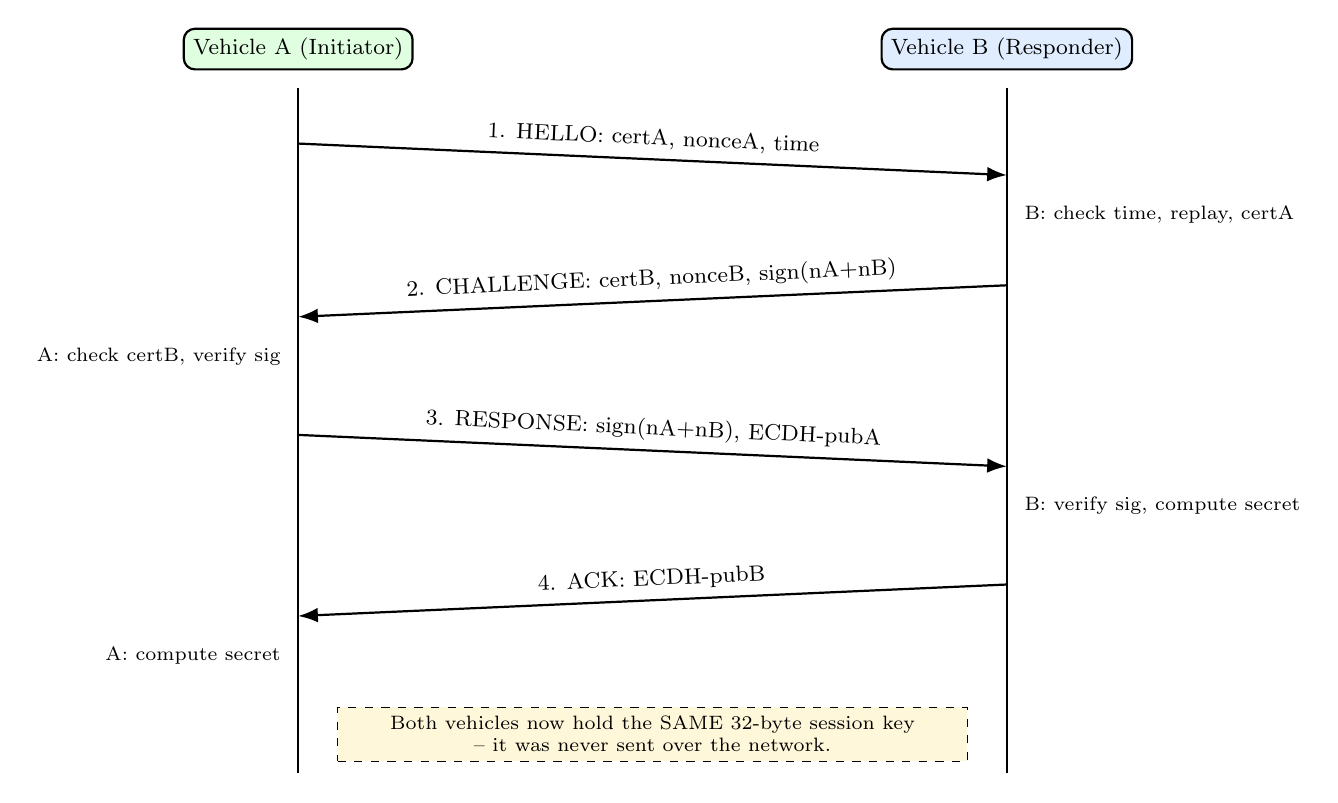
\begin{tikzpicture}[font=\footnotesize]
  % lifelines
  \node[draw,thick,rounded corners,fill=green!12] (A) at (0,0)
       {Vehicle A (Initiator)};
  \node[draw,thick,rounded corners,fill=boxblue] (B) at (9,0)
       {Vehicle B (Responder)};
  \draw[thick] (0,-0.5) -- (0,-9.2);
  \draw[thick] (9,-0.5) -- (9,-9.2);
  % step 1
  \draw[-{Latex[length=2.5mm]},thick] (0,-1.2) -- (9,-1.6)
       node[midway,above,sloped]{1. HELLO: certA, nonceA, time};
  \node[right=1mm,align=left,font=\scriptsize] at (9,-2.1)
       {B: check time, replay, certA};
  % step 2
  \draw[-{Latex[length=2.5mm]},thick] (9,-3.0) -- (0,-3.4)
       node[midway,above,sloped]{2. CHALLENGE: certB, nonceB, sign(nA+nB)};
  \node[left=1mm,align=right,font=\scriptsize] at (0,-3.9)
       {A: check certB, verify sig};
  % step 3
  \draw[-{Latex[length=2.5mm]},thick] (0,-4.9) -- (9,-5.3)
       node[midway,above,sloped]{3. RESPONSE: sign(nA+nB), ECDH-pubA};
  \node[right=1mm,align=left,font=\scriptsize] at (9,-5.8)
       {B: verify sig, compute secret};
  % step 4
  \draw[-{Latex[length=2.5mm]},thick] (9,-6.8) -- (0,-7.2)
       node[midway,above,sloped]{4. ACK: ECDH-pubB};
  \node[left=1mm,align=right,font=\scriptsize] at (0,-7.7)
       {A: compute secret};
  % result
  \node[draw,dashed,fill=boxyellow,minimum width=8cm,align=center,font=\scriptsize]
       at (4.5,-8.7)
       {Both vehicles now hold the SAME 32-byte session key\\
        -- it was never sent over the network.};
\end{tikzpicture}
\end{center}

\subsection{Diagram 2 --- The three gates every handshake message passes}
\begin{center}
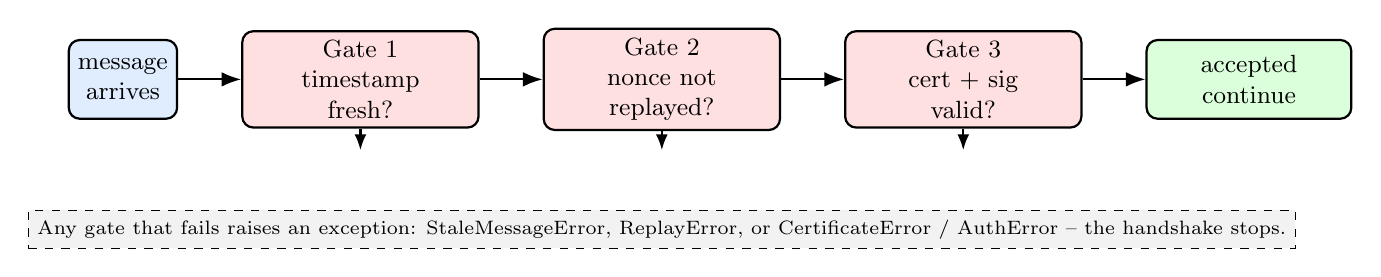
\begin{tikzpicture}[font=\small,node distance=7mm,
   gate/.style={draw,thick,rounded corners,minimum width=3.0cm,minimum height=1.0cm,
                align=center,fill=red!12},
   ok/.style={draw,thick,rounded corners,minimum width=2.6cm,minimum height=1.0cm,
              align=center,fill=green!14}]
  \node[draw,thick,rounded corners,fill=boxblue,minimum height=1cm,align=center] (in) {message\\arrives};
  \node[gate,right=8mm of in] (g1) {Gate 1\\timestamp\\fresh?};
  \node[gate,right=8mm of g1] (g2) {Gate 2\\nonce not\\replayed?};
  \node[gate,right=8mm of g2] (g3) {Gate 3\\cert + sig\\valid?};
  \node[ok,right=8mm of g3] (acc) {accepted\\continue};
  \draw[-{Latex[length=2.5mm]},thick] (in) -- (g1);
  \draw[-{Latex[length=2.5mm]},thick] (g1) -- (g2);
  \draw[-{Latex[length=2.5mm]},thick] (g2) -- (g3);
  \draw[-{Latex[length=2.5mm]},thick] (g3) -- (acc);
  \node[below=10mm of g2,draw,dashed,fill=gray!10,minimum width=9cm,
        align=center,font=\scriptsize]
       {Any gate that fails raises an exception: StaleMessageError,
        ReplayError, or CertificateError / AuthError -- the handshake stops.};
  \draw[-{Latex[length=2mm]},thick] (g1) -- ++(0,-0.9);
  \draw[-{Latex[length=2mm]},thick] (g2) -- ++(0,-0.9);
  \draw[-{Latex[length=2mm]},thick] (g3) -- ++(0,-0.9);
\end{tikzpicture}
\end{center}

% =====================================================================
\section{Presentation Pack}
% =====================================================================

\subsection{Slide Outline}

\textbf{Slide 1 --- Why a Handshake?}
\begin{itemize}
  \item Before any safety message, the cars must trust each other.
  \item Showing a certificate is not enough --- certificates are public.
  \item The handshake adds a live ``prove you own the key'' test.
  \item It also secretly agrees on a shared encryption key.
\end{itemize}

\textbf{Slide 2 --- The Four Steps.}
\begin{itemize}
  \item HELLO: A sends its certificate + a random nonce.
  \item CHALLENGE: B sends its certificate + nonce + a signature.
  \item RESPONSE: A sends its signature + an ECDH public key.
  \item ACK: B sends its ECDH public key --- done.
\end{itemize}

\textbf{Slide 3 --- Challenge--Response: Proving Key Ownership.}
\begin{itemize}
  \item Each side signs the pair of fresh nonces with its private key.
  \item The other side verifies with the certificate's public key.
  \item A valid signature over a brand-new nonce = ``you own the key, now''.
  \item Wrong/missing key $\to$ \texttt{AuthError} --- impersonation caught.
\end{itemize}

\textbf{Slide 4 --- Three Gates Stop Replay.}
\begin{itemize}
  \item Timestamp gate: message older than 5\,s $\to$ \texttt{StaleMessageError}.
  \item Nonce gate: nonce seen before $\to$ \texttt{ReplayError}.
  \item Certificate gate: not CA-signed $\to$ \texttt{CertificateError}.
  \item Belt-and-braces: cheap time check plus exact-duplicate check.
\end{itemize}

\textbf{Slide 5 --- A Shared Key, Never Sent.}
\begin{itemize}
  \item Each side makes an ephemeral ECDH key pair.
  \item Public halves are swapped in RESPONSE and ACK.
  \item Both compute the same secret; HKDF turns it into a 32-byte key.
  \item Ephemeral keys $\to$ forward secrecy. ``Keys match: True''.
\end{itemize}

\subsection{Speaker Talking Points (about 30--60 seconds each)}

\textbf{Slide 1.} ``Before our two cars send a single safety message, they run a
handshake --- a short, fixed four-step conversation. Why bother? Because simply
showing a certificate is not enough. A certificate is public; anyone can copy it.
So the handshake does two extra jobs. First, it makes each car prove, live, that
it actually \emph{owns} the private key behind its certificate --- not just that
it has a copy of the certificate. Second, while doing that, the two cars secretly
agree on a shared encryption key. By the end, each car is certain who it is
talking to and they share a secret nobody else knows.''

\textbf{Slide 2.} ``The handshake has four messages. In HELLO, car A introduces
itself, sending its certificate and a fresh random number called a nonce. In
CHALLENGE, car B replies with its own certificate, its own nonce, and --
importantly -- a digital signature over both nonces. In RESPONSE, car A signs
both nonces too and includes a special temporary key for the key exchange.
Finally in ACK, car B sends its matching temporary key. Four messages: two to
swap certificates, and the signatures going both ways for the proof.''

\textbf{Slide 3.} ``The heart of the handshake is challenge--response. Each car
picks a brand-new random nonce that the other side could not have predicted. Each
car then signs the pair of nonces with its private key. The other side verifies
that signature using the public key inside the certificate. Here is the clever
part: because the nonce is fresh, a recorded old signature is useless, and
because signing needs the private key, only the genuine car can produce a
signature that verifies. If the signature is wrong, our code raises an AuthError
and says `possible impersonation'. That single check is what stops a fake car.''

\textbf{Slide 4.} ``Every handshake message passes three gates. The first gate
checks the timestamp --- if the message is more than five seconds old, it is
stale and rejected immediately; that is cheap and fast. The second gate checks
the nonce against a replay cache --- if we have seen that exact nonce before, it
is a replay and we reject it. The third gate checks the certificate is signed by
our trusted CA. Any gate failing throws a specific exception and the handshake
stops. Two of those gates --- timestamp and nonce --- together make replaying an
old handshake impossible.''

\textbf{Slide 5.} ``Finally, the key. During the handshake each car generates a
temporary, throw-away key pair for something called ECDH. They swap only the
\emph{public} halves, inside the RESPONSE and ACK messages. Then each car
combines its own private half with the other's public half, and thanks to the
maths both end up with the \emph{same} secret --- even though that secret was
never sent. HKDF turns it into a clean 32-byte key. And because those ECDH keys
are thrown away after the session, even a key stolen later cannot unlock this
conversation --- that is forward secrecy. The demo ends by printing `Keys match:
True'.''

\subsection{Live-Demo Script}
\begin{enumerate}
  \item \textbf{Set up.} Run \texttt{ca.py} and the two \texttt{issue\_cert.py}
        commands so the certificates exist.
  \item \textbf{Run the handshake.} Execute \texttt{python
        protocol\textbackslash auth\_protocol.py}. Read the log aloud, pointing
        at each of the four steps in turn.
  \item \textbf{Point at the proof lines.} ``Certificate VALID'' (the cert gate)
        and ``signature verified'' (the challenge--response).
  \item \textbf{Point at the result.} ``Keys match: True'' --- ``the same key on
        both sides, never sent over the wire.''
  \item \textbf{Break it live.} Apply Experiment~1 (replay) or Experiment~3 (bad
        signature) from the Hands-On section and show the \texttt{ReplayError} or
        \texttt{AuthError}. Restore the file afterwards.
\end{enumerate}

\subsection{Examiner Q\&A}
\begin{enumerate}
  \item \textbf{Q: What is mutual authentication and why not just one-sided?}\\
        A: Both parties prove identity to each other. One-sided authentication
        leaves the unchecked side open to impersonation and enables a
        man-in-the-middle; mutual authentication checks both directions.
  \item \textbf{Q: A certificate is already trusted --- why also do
        challenge--response?}\\
        A: A certificate is public and can be copied. The challenge--response
        forces the sender to sign a \emph{fresh, unpredictable} nonce with the
        private key, proving it \emph{owns} the key right now, not just holds a
        copy of the certificate.
  \item \textbf{Q: Why are there two nonces, one from each side?}\\
        A: So that \emph{each} side issues a challenge the \emph{other} must
        answer. Both nonces are signed, giving a two-way proof, and both feed
        HKDF so the session key is bound to this exact exchange.
  \item \textbf{Q: How does the handshake stop a replayed HELLO?}\\
        A: Two ways: \texttt{TimestampValidator} rejects it if older than 5\,s,
        and \texttt{ReplayCache} rejects it if its nonce was already seen
        (remembered for 300\,s).
  \item \textbf{Q: How is the session key the same on both sides if it is never
        sent?}\\
        A: ECDH: each side combines its ephemeral private key with the peer's
        ephemeral public key to get the identical shared secret; both then run
        HKDF with the same nonce order, producing the identical 32-byte key.
  \item \textbf{Q: Where does forward secrecy come from in the handshake?}\\
        A: The ECDH key pairs are \emph{ephemeral} --- generated by
        \texttt{generate\_ecdh\_keypair} for this session and discarded.
        A later theft of the long-term certificate key cannot rebuild them.
  \item \textbf{Q: What exception is raised for a forged signature, and where?}\\
        A: \texttt{ecdsa\_verify} returns \texttt{False}, and
        \texttt{process\_challenge} (or \texttt{process\_response}) raises
        \texttt{AuthError} --- ``Challenge signature invalid, possible
        impersonation''.
  \item \textbf{Q: Name a limitation of this handshake.}\\
        A: It needs clocks synchronised within 5\,s, so heavy clock skew could
        reject an honest handshake; the ACK has no timestamp field, so it is not
        freshness-checked; and the parameter \texttt{original\_hello} in
        \texttt{process\_response} is passed but unused. Networking is added
        separately in S6.
\end{enumerate}

% =====================================================================
\section{Glossary}
% =====================================================================
\begin{description}[style=nextline,leftmargin=0pt]
  \item[Handshake] A short fixed exchange of messages that sets up a secure session.
  \item[Authentication] Proving who you are.
  \item[Mutual authentication] Both parties prove identity to each other.
  \item[Initiator] The vehicle that starts the handshake (sends HELLO).
  \item[Responder] The vehicle that answers the handshake.
  \item[Challenge--response] A test: send a fresh value, demand an operation only
        the genuine party can perform.
  \item[Nonce] A fresh single-use random value (here 32 bytes, as hex).
  \item[HELLO] Step 1 message: certificate + nonce + timestamp.
  \item[CHALLENGE] Step 2 message: certificate + nonce + signature + timestamp.
  \item[RESPONSE] Step 3 message: signature + ECDH public key + timestamp.
  \item[ACK] Step 4 message: ECDH public key, completing the handshake.
  \item[ReplayCache] A store of seen nonces that rejects duplicates.
  \item[TimestampValidator] A check that rejects messages older (or newer) than 5\,s.
  \item[Replay attack] Re-sending a previously captured valid message.
  \item[Stale message] A message whose timestamp is outside the allowed window.
  \item[Dataclass] A Python class that simply holds named fields.
  \item[JSON] A text format for structured data, used as the wire format.
  \item[Serialization] Converting an object to bytes/text for sending.
  \item[ECDH] Elliptic-Curve Diffie--Hellman key exchange.
  \item[Ephemeral key] A key generated for one session then discarded.
  \item[HKDF] The key-derivation function turning the shared secret into the key.
  \item[Session key] The shared 32-byte AES key produced by the handshake.
  \item[Forward secrecy] Past sessions stay secret even if a key leaks later.
  \item[AuthError] This project's exception for a failed authentication step.
  \item[ReplayError] Exception raised by the ReplayCache for a repeated nonce.
  \item[StaleMessageError] Exception raised for an out-of-window timestamp.
  \item[CertificateError] Exception raised when certificate verification fails.
  \item[tbs\_certificate\_bytes] The ``to-be-signed'' body bytes of a certificate.
\end{description}

% =====================================================================
\section{References and Further Study}
% =====================================================================
\begin{itemize}
  \item \textbf{Mutual authentication (Wikipedia)} ---
        \url{https://en.wikipedia.org/wiki/Mutual_authentication}\\
        Read for: why both sides must authenticate.
  \item \textbf{Challenge--response authentication (Wikipedia)} ---
        \url{https://en.wikipedia.org/wiki/Challenge%E2%80%93response_authentication}\\
        Read for: the core idea behind the nonce + signature proof.
  \item \textbf{Cryptographic nonce (Wikipedia)} ---
        \url{https://en.wikipedia.org/wiki/Cryptographic_nonce}\\
        Read for: why a fresh single-use value defeats replay.
  \item \textbf{Replay attack (Wikipedia)} ---
        \url{https://en.wikipedia.org/wiki/Replay_attack}\\
        Read for: the attack the ReplayCache and TimestampValidator block.
  \item \textbf{TLS 1.3 handshake (RFC 8446 --- read Section 2)} ---
        \url{https://datatracker.ietf.org/doc/html/rfc8446}\\
        Read for: a real-world handshake using the same ideas (certificates,
        signatures, ephemeral key exchange).
  \item \textbf{Diffie--Hellman key exchange (Wikipedia)} ---
        \url{https://en.wikipedia.org/wiki/Diffie%E2%80%93Hellman_key_exchange}\\
        Read for: how both sides reach the same secret without sending it.
  \item \textbf{Forward secrecy (Wikipedia)} ---
        \url{https://en.wikipedia.org/wiki/Forward_secrecy}\\
        Read for: why ephemeral handshake keys matter.
  \item \textbf{Python dataclasses documentation} ---
        \url{https://docs.python.org/3/library/dataclasses.html}\\
        Read for: how the four message classes work.
  \item \textbf{Python json module documentation} ---
        \url{https://docs.python.org/3/library/json.html}\\
        Read for: \texttt{json.dumps} / \texttt{json.loads} used by
        \texttt{to\_json} / \texttt{from\_json}.
  \item \textbf{Python cryptography --- elliptic-curve docs} ---
        \url{https://cryptography.io/en/latest/hazmat/primitives/asymmetric/ec/}\\
        Read for: the ECDH and ECDSA calls the handshake relies on.
  \item \textbf{NIST SP 800-63B --- authentication guidance} ---
        \url{https://pages.nist.gov/800-63-3/sp800-63b.html}\\
        Read for: professional terminology around authentication and replay.
\end{itemize}

\vfill
\begin{center}\footnotesize\itshape
End of Section S4. The handshake's output --- the session key --- is consumed by
S5 (Secure Messaging).
\end{center}

\end{document}
